Metode \textit{Synthetic Minority Over-sampling Technique} (SMOTE)
\cite{chawla2002smote} menggunakan pendekatan \textit{over-sampling} yang mana
kelas minoritas ditambah dengan membuat sampel sintetis bukan dengan
mengganti sampel dari kelas mayoritas menjadi kelas minoritas.
Sampel sintetis dibuat lewat aplikasi, dengan beroperasi pada
ruang fitur bukan pada ruang data.
Kelas minoritas ditambah dengan mengambil setiap sampel-sampel dari kelas
minoritas dan membuat sampel sintetis diantara segmen garis yang menggabungkan
setiap/semua \textit{k-nearest-neighbors} dari kelas minoritas.
Bergantung kepada jumlah \textit{over-sampling} yang dibutuhkan, instan dari
\textit{k-nearest-neighbors} dipilih secara acak.

\begin{figure}[htbp]
\centering
\setlength\fboxsep{4pt}
\fbox{
	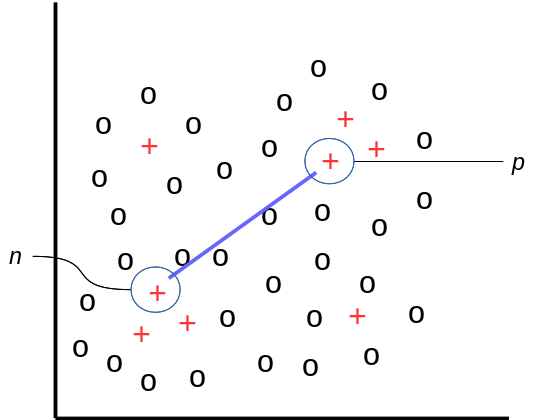
\includegraphics[keepaspectratio=true,scale=0.35]{SMOTE-example}
}
	\caption{Ilustrasi pembuatan sampel sintetis pada SMOTE.
	\textit{p} adalah sampel minoritas, \textit{n} adalah salah satu
	\textit{k-nearest-neighbors} dari \textit{p}.
	Sampel sintetis yang baru akan berada digaris antara \textit{p} dan
	\textit{n}.
	}
	\label{fig:smote}
\end{figure}

Sampel sintetis dibuat dengan cara berikut,
\begin{compactitem}%
	\item Hitung selisih antara vektor fitur (sampel) dengan tetangga
	terdekatnya.
	\item Kalikan selisih tersebut dengan angka ril acak antara 0 sampai 1,
	dan
	\item tambahkan hasilnya ke vektor fitur.
\end{compactitem}

Cara ini membuat sampel secara acak pada segmen garis antara dua fitur yang
terpilih, seperti yang terlihat pada gambar \ref{fig:smote}.
Pendekatan ini secara efektif mendorong wilayah pembelajaran dari kelas
minoritas menjadi lebih besar tanpa menyebabkan \textit{overfitting}.

Ambil contoh sebuah sampel (6,4) dan (4,3) sebagai tetangga terdekatnya.
(6,4) adalah sampel yang akan dicari \textit{k-nearest-neighbors}-nya.
(4,3) adalah salah satu dari \textit{k-nearest-neighbors}-nya.
Misalkan,
\[
\begin{matrix}
f1_1 = 6 & f1_2 = 4 \\
f2_1 = 4 & f2_2 = 3
\end{matrix}
\]
\[
\begin{matrix}
f2_1 - f1_1 = 4 - 6 = -2 \\
f2_2 - f1_2 = 3 - 4 = -1
\end{matrix}
\]

Sampel baru dihasilkan dengan,
\[
(f1', f2') = (6,4) + random(0-1) * (-2,-1)
\]

Fungsi \textit{random(0-1)} menghasilkan bilangan ril acak dari 0 sampai 1.
